\documentclass[aspectratio=169,11pt]{beamer}
\usetheme{Madrid}
\usecolortheme{seahorse}
\usepackage{booktabs}
\usepackage{graphicx}
\usepackage{amsmath}
\usepackage{xcolor}
\usepackage{pgfpages}

\definecolor{mblue}{RGB}{0,91,161}
\definecolor{mred}{RGB}{196,30,58}
\definecolor{mgray}{RGB}{100,100,100}

\setbeamertemplate{navigation symbols}{}
\setbeamertemplate{footline}[frame number]

% To compile speaker notes as a separate PDF, change to:
%   \setbeameroption{show only notes}
% To present with notes on a second screen:
%   \setbeameroption{show notes on second screen=right}
\setbeameroption{hide notes}

\title{A Statistical Audit of LLM Calibration\\Heterogeneity Across Knowledge Domains}
\author{Jennifer Zhang}
\institute{STAT 215B, Spring 2026}
\date{}

\begin{document}

\maketitle
\note{}

% ============================================================
%  1. MOTIVATION
% ============================================================

\begin{frame}{What is calibration — and why does it matter?}
A model is \textbf{well-calibrated} if its stated confidence tracks empirical accuracy:
\begin{itemize}
  \item 80\% confident $\Rightarrow$ correct 80\% of the time
\end{itemize}

\vspace{0.5em}
Miscalibration is typically reported as a \textbf{single number} (Expected Calibration Error):
\[
  \mathrm{ECE} = \sum_b \frac{|B_b|}{n}\,|\text{acc}(B_b) - \text{conf}(B_b)|
\]

\vspace{0.5em}
\textbf{The problem:} aggregate ECE over 57 subjects, 4 domains, 14{,}042 questions
hides \emph{where} and \emph{how much} miscalibration occurs.

\vspace{0.5em}
\textbf{Analogy:} reporting one accuracy number across demographic groups is
insufficient for a fairness audit. The same logic applies to calibration.
\end{frame}
\note{
  \textbf{[~45 sec]}

  Open with the definition — make sure the audience knows what calibration means
  before anything else. The formula is on the slide so you don't need to dwell on it;
  just say ``ECE is the weighted average gap between confidence and accuracy across
  confidence bins.''

  The key move is the fairness analogy: just like we'd never accept a single accuracy
  number as a fairness audit, a single ECE number is not a calibration audit.
  Land that point before moving on — it's the whole motivation.

  If anyone in the room works on ML deployment, you can add: ``when a model says
  it's 90\% confident, users treat that as a reliability signal — if that signal is
  only accurate on average, users in certain domains are being systematically misled.''
}

% ------------------------------------------------------------

\begin{frame}{Research questions}
\begin{enumerate}
  \item \textbf{How much} of calibration variance is attributable to domain vs.\ subject
    vs.\ individual question?
  \item \textbf{What question features} predict the direction and magnitude of
    miscalibration?
  \item \textbf{Are patterns consistent} across models, or model-specific?
\end{enumerate}

\vspace{1em}
\begin{block}{Framework}
  Three-level mixed model + isotonic calibration curves + empirical Bayes shrinkage
  + Benjamini--Hochberg FDR correction
\end{block}
\end{frame}
\note{
  \textbf{[~30 sec]}

  Read the three questions quickly — the audience will follow.
  For the framework block: ``I won't spend time on each method now; the key idea is
  that we want statistically rigorous answers, not just descriptive bar charts.''

  Don't explain what BH correction is here — that comes up naturally in the
  robustness slide. Just name-drop it so the audience knows it's coming.
}

% ============================================================
%  2. DATA & METHOD
% ============================================================

\begin{frame}{Data \& confidence elicitation}
\textbf{MMLU}: 14{,}042 four-choice questions, 57 subjects, 4 domains
\hfill{\small\color{mgray}(questions $\to$ subjects $\to$ domains)}

\vspace{1em}
\textbf{Two models:}
\begin{itemize}
  \item \textbf{GPT-4o-mini} (OpenAI API, \texttt{top\_logprobs=20})
  \item \textbf{Llama-3-8B-Instruct} (Colab T4, 4-bit quantization)
\end{itemize}

\vspace{1em}
\textbf{Confidence measure} — renormalized softmax over the four answer tokens:
\[
  c_i = \max_{a \in \{A,B,C,D\}} \frac{e^{\ell_a}}{\sum_{a'} e^{\ell_{a'}}}
\]

\vspace{0.5em}
\textbf{Primary outcome} — signed calibration gap:
\[
  \mathrm{gap}_i = c_i - y_i \quad (y_i \in \{0,1\})
\]
Positive = overconfident; negative = underconfident.
\end{frame}
\note{
  \textbf{[~45 sec]}

  Explain the hierarchy briefly: ``MMLU has 57 subjects like clinical medicine,
  formal logic, high school math — grouped into 4 broad domains. That nested structure
  is what makes a multilevel model the right tool.''

  For the confidence measure: ``We extract the log probability the model assigns to
  each of the four answer tokens, renormalize them to sum to 1, and take the max.
  This is a standard approach — it gives us a proper probability on the model's
  chosen answer.''

  For the signed gap: ``The nice thing about using the signed gap instead of ECE is
  that it tells us the \emph{direction} — positive means the model thinks it knows
  more than it does.''

  One methodological note if it comes up: we had to use top\_logprobs=20 for GPT
  because with 5 logprobs, 55\% of questions had at least one answer token missing,
  which would artificially inflate confidence estimates. That's a real data quality
  issue that took some debugging.
}

% ============================================================
%  3. CORE FINDINGS
% ============================================================

\begin{frame}{Finding 1: heterogeneity is real but concentrated at the question level}

\begin{columns}[T]
  \begin{column}{0.48\textwidth}
    \begin{table}
      \small
      \caption{Variance decomposition (GPT-4o-mini)}
      \begin{tabular}{lrr}
        \toprule
        Level & Variance & ICC \\
        \midrule
        Domain   & 0.000 & 0.000 \\
        Subject  & 0.013 & \textbf{0.079} \\
        Residual & 0.150 & 0.922 \\
        \bottomrule
      \end{tabular}
    \end{table}

    \vspace{0.5em}
    \small
    \textbf{7.9\%} of total calibration variance is between-subject --- not noise,
    but not dominant either.

    \vspace{0.5em}
    Domain variance $= 0$: only 4 groups; unidentifiable with REML.
  \end{column}
  \begin{column}{0.48\textwidth}
    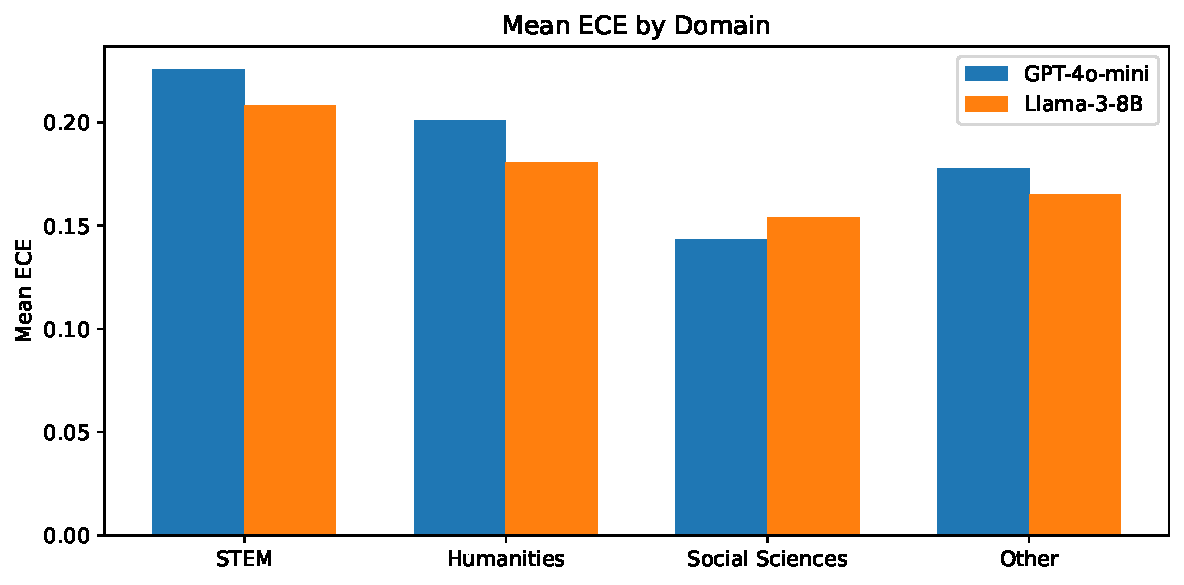
\includegraphics[width=\textwidth]{figures/domain_ece.pdf}
    \small\color{mgray} Domain-level mean ECE (descriptive only)
  \end{column}
\end{columns}
\end{frame}
\note{
  \textbf{[~30 sec]}

  Lead with the 7.9\% number: ``92\% of the variance is at the question level —
  individual questions are noisy. But 7.9\% is systematically concentrated at the
  subject level, meaning some subjects are persistently harder to be calibrated on.
  That's not just noise — it's structure.''

  Be upfront about domain ICC = 0: ``With only 4 domain groups the model can't
  estimate domain-level variance reliably — that's a limitation. We treat domain as
  a descriptive label here, not a modeled random effect.''

  The bar chart on the right is descriptive — Humanities has noticeably higher ECE.
  Point to it briefly as motivation for the next slide.
}

% ------------------------------------------------------------

\begin{frame}{Finding 2: calibration curves reveal systematic overconfidence}
  \begin{center}
    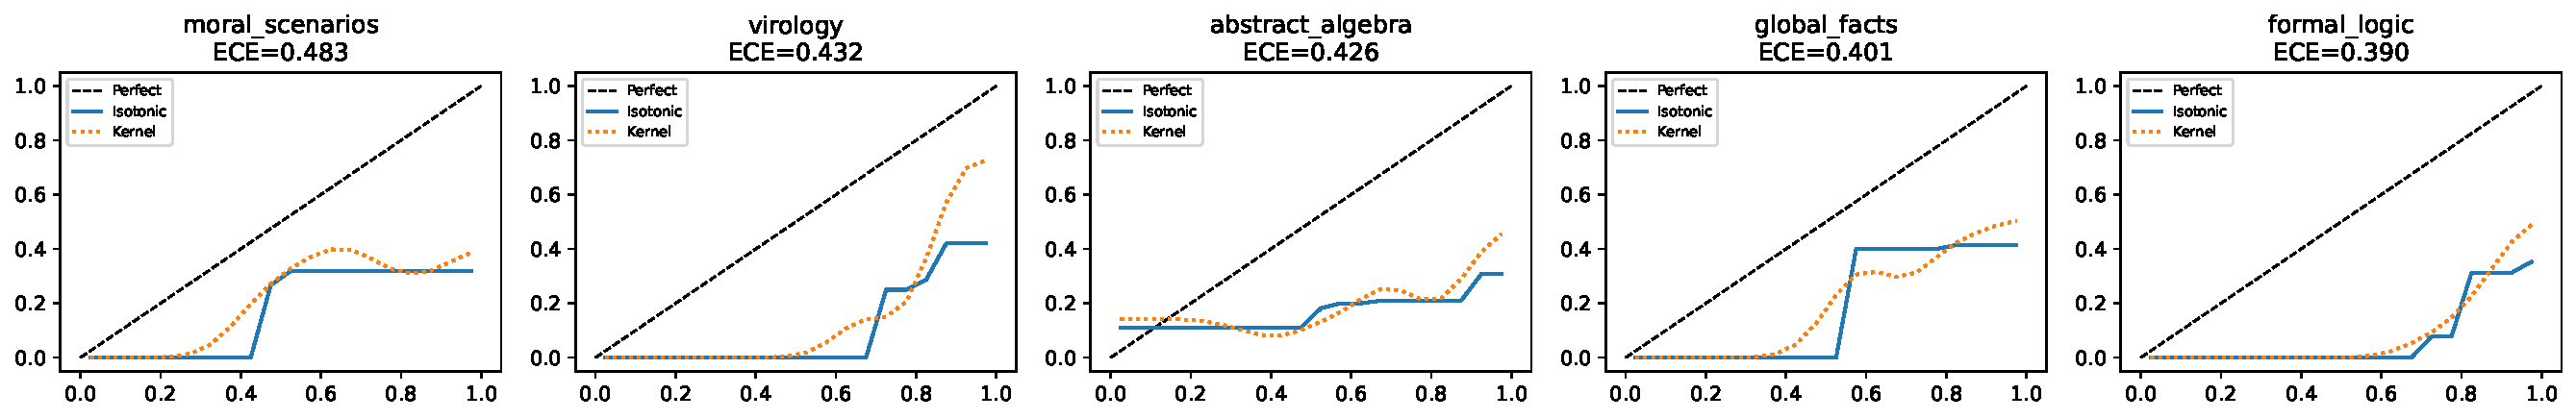
\includegraphics[width=0.85\textwidth]{figures/top5_miscalibrated_gpt4o.pdf}
  \end{center}
  \vspace{-0.5em}
  {\small Reliability curves (isotonic = solid, kernel = dashed) for the 5 most
  miscalibrated subjects. All five lie \emph{below} the diagonal — stated confidence
  exceeds empirical accuracy throughout.}
\end{frame}
\note{
  \textbf{[~30 sec]}

  Point to the diagonal: ``A perfectly calibrated model sits on this line.
  Every one of these subjects is below it — the model is consistently more confident
  than it is accurate.''

  Point out the isotonic vs. kernel agreement: ``The solid and dashed lines track
  each other closely, which validates that the monotonicity assumption in isotonic
  regression isn't distorting the picture.''

  Name the subjects briefly if time allows: ``Moral scenarios, formal logic,
  abstract algebra, professional law — these are subjects requiring abstract or
  normative reasoning, not factual recall. The model's RLHF training likely skews
  toward more applied content.''

  Keep this slide fast — the next one has the more striking quantitative result.
}

% ------------------------------------------------------------

\begin{frame}{Finding 3: universal overconfidence, 13$\times$ range in magnitude}
  \begin{columns}[T]
    \begin{column}{0.62\textwidth}
      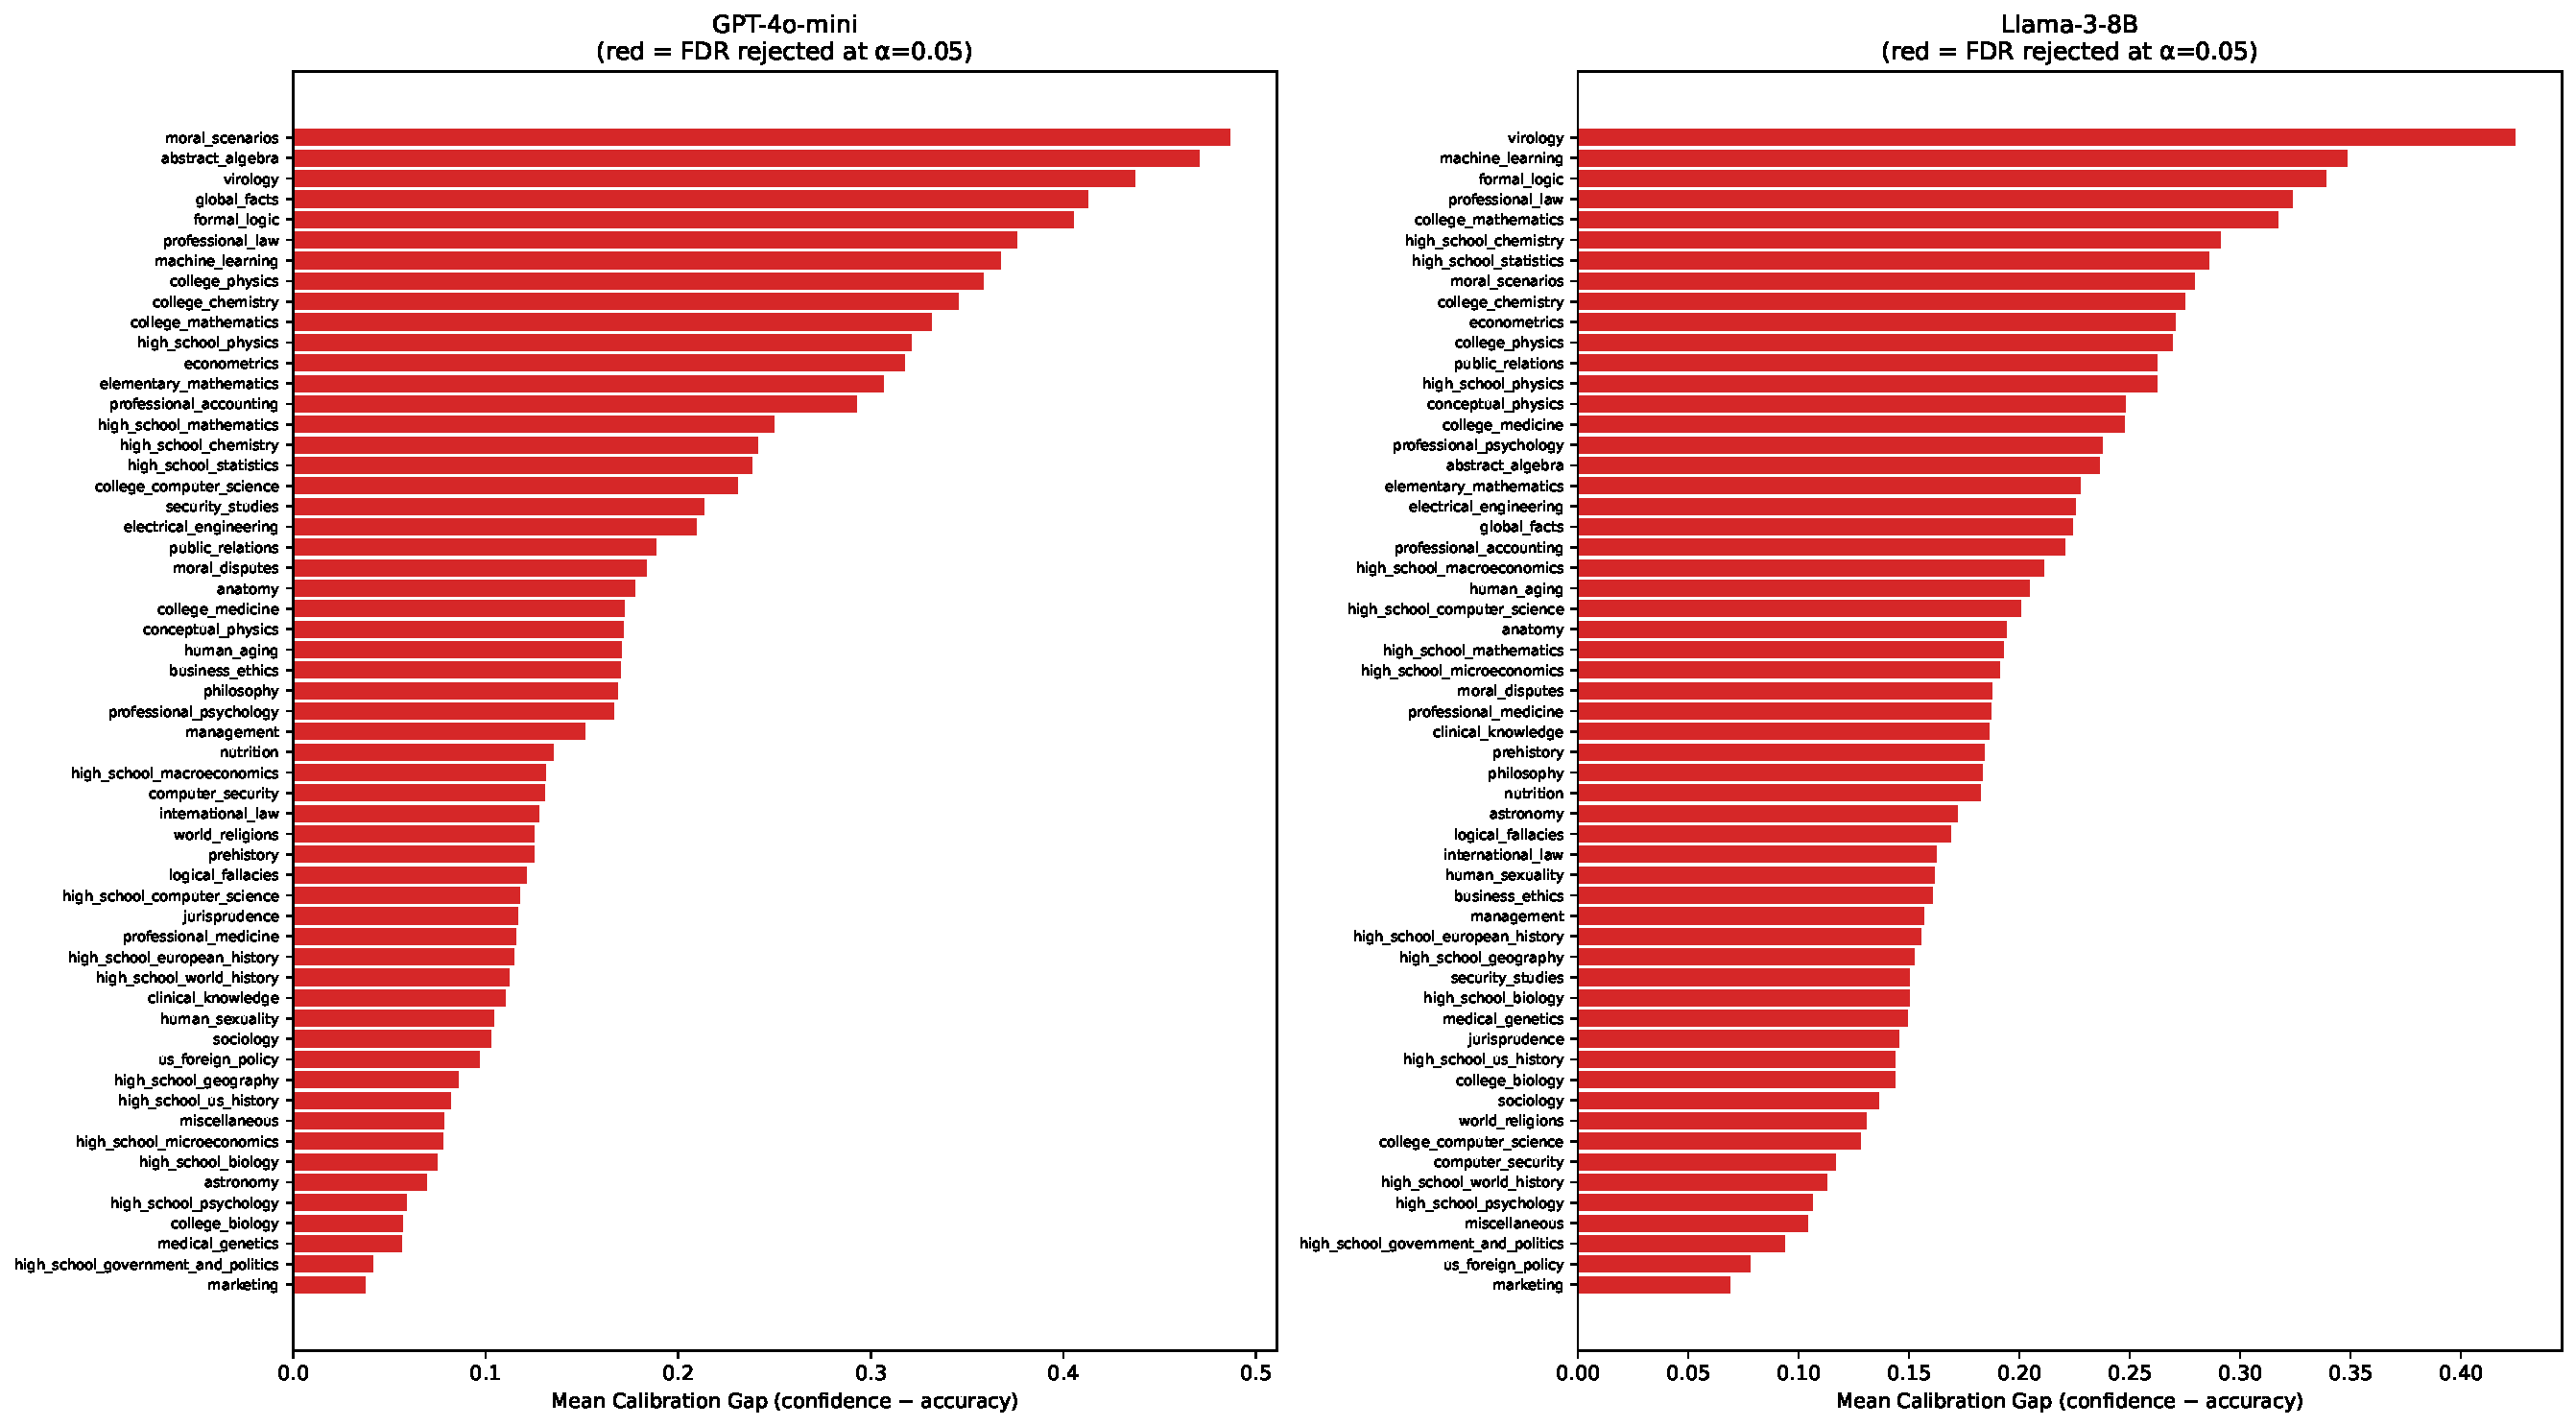
\includegraphics[width=\textwidth]{figures/subject_mean_gap.pdf}
    \end{column}
    \begin{column}{0.35\textwidth}
      \small
      \textbf{57/57 subjects} rejected after BH correction ($\alpha = 0.05$).

      \vspace{0.8em}
      But the \emph{magnitude} varies drastically:
      \begin{itemize}
        \item \textbf{Max}: moral scenarios (0.487)
        \item \textbf{Min}: marketing (0.037)
        \item \textbf{Range}: 13$\times$
      \end{itemize}

      \vspace{0.8em}
      Humanities subjects cluster at the top; STEM and ``Other'' at the bottom.

      \vspace{0.8em}
      {\color{mgray}\small Intercept $= 0.196$ ($p < 0.001$); overconfidence is a
      baseline effect of RLHF fine-tuning.}
    \end{column}
  \end{columns}
\end{frame}
\note{
  \textbf{[~45 sec]}

  Preempt the obvious question: ``You might wonder if 57/57 is a meaningful result
  or just an artifact of large sample sizes. It's largely the latter in terms of the
  binary reject/fail-to-reject — with 14,000 questions, you'll detect almost anything.
  But that's not the interesting finding. The interesting finding is the 13-fold range
  in magnitude.''

  ``A gap of 0.487 on moral scenarios means the model is, on average, nearly 50
  percentage points more confident than it is accurate. A gap of 0.037 on marketing
  means it's essentially well-calibrated. Those are qualitatively different situations
  that a single aggregate ECE number cannot distinguish.''

  If asked why 57/57: the intercept of 0.196 is large relative to per-subject
  standard errors (~0.025), giving t-statistics around 8 for the average subject.
  BH adjusts for 57 tests but p-values are still near zero. The sensitivity analysis
  slide will confirm this isn't sensitive to the alpha choice.
}

% ------------------------------------------------------------

\begin{frame}{What predicts the gap? Fixed effects}
  \begin{columns}[T]
    \begin{column}{0.48\textwidth}
      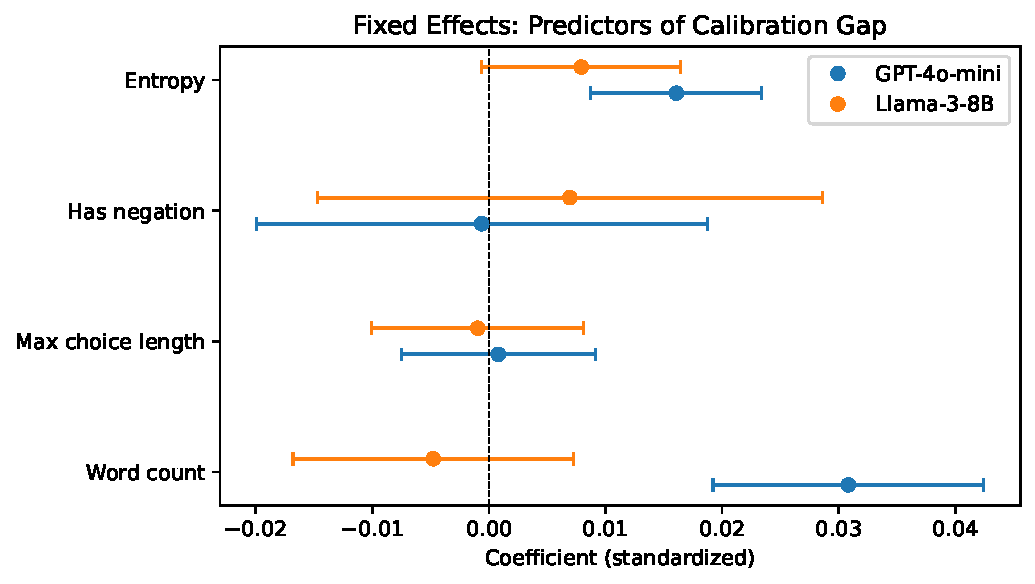
\includegraphics[width=\textwidth]{figures/coef_plot.pdf}
    \end{column}
    \begin{column}{0.48\textwidth}
      \small
      \begin{itemize}
        \item \textbf{Word count} ($\hat\beta = 0.031$, $p < 0.001$): longer questions
          $\Rightarrow$ larger gap
        \item \textbf{Entropy} ($\hat\beta = 0.016$, $p < 0.001$): when model spreads
          probability across options, gap \emph{increases} --- counterintuitive
        \item \textbf{Max option length}, \textbf{negation}: not significant
      \end{itemize}

      \vspace{0.8em}
      Entropy result: the model doesn't reliably correct confidence when uncertain.
      Distributing probability $\neq$ being right more often.
    \end{column}
  \end{columns}
\end{frame}
\note{
  \textbf{[~30 sec]}

  The entropy finding is the most interesting one to discuss: ``Intuitively you'd
  expect that when the model spreads its probability mass across options — expressing
  uncertainty — the gap would shrink. But it goes the other way. Higher entropy
  is associated with \emph{larger} gaps. The model isn't reliably correct more often
  when it's hedging; it's just miscalibrated in a different way.''

  Word count is less surprising: ``Longer, more complex questions are harder, and
  the model doesn't adjust its confidence accordingly.''

  Negation being non-significant is worth a brief mention if asked: we expected
  ``not/except/never'' questions to trip up the model, but they don't show up after
  controlling for length and entropy.
}

% ============================================================
%  4. ROBUSTNESS
% ============================================================

\begin{frame}{Sensitivity analysis: are findings robust?}

\textbf{Three stress tests on GPT-4o-mini results.}

\vspace{0.8em}
\begin{columns}[T]
  \begin{column}{0.32\textwidth}
    \textbf{1. ECE bin count}\\[0.4em]
    \small
    Recompute subject ECE at $b \in \{10, 15, 20, 25, 30\}$ bins.\\[0.4em]
    Spearman $\rho \geq 0.997$ vs.\ baseline for all $b$.\\[0.4em]
    \textbf{Rankings are stable.}
  \end{column}
  \begin{column}{0.32\textwidth}
    \textbf{2. FDR threshold}\\[0.4em]
    \small
    Apply BH at $\alpha \in \{0.01, 0.05, 0.10\}$.\\[0.4em]
    $\alpha = 0.01$: 56/57 rejected\\
    $\alpha = 0.05$: 57/57 rejected\\
    $\alpha = 0.10$: 57/57 rejected\\[0.4em]
    \textbf{Not driven by $\alpha$ choice.}
  \end{column}
  \begin{column}{0.32\textwidth}
    \textbf{3. Model structure}\\[0.4em]
    \small
    Compare 3-level (domain + subject) to 2-level (subject only).\\[0.4em]
    ICC$_\text{subject} = 0.079$ in both; $\hat\sigma^2_\text{subject}$ identical.\\[0.4em]
    \textbf{ICC estimate is robust.}
  \end{column}
\end{columns}

\vspace{0.8em}
\small\color{mgray}
\textit{Note:} Llama-3-8B-Instruct cross-model results are pending a verified re-run;
cross-model comparisons are preliminary.
\end{frame}
\note{
  \textbf{[~60 sec] — spend real time here}

  Frame this section: ``Before I trust any of these findings, I want to know whether
  they're artifacts of specific choices I made. I ran three stress tests.''

  Column 1 (ECE bins): ``ECE depends on how you bin confidence scores. I tried
  10 to 30 bins — the Spearman rank correlation of subject rankings stays above 0.997.
  The top-5 miscalibrated subjects don't move.''

  Column 2 (FDR threshold): ``You might wonder if 57/57 only holds at alpha=0.05.
  At the stricter alpha=0.01, it's still 56/57. The finding is not sensitive to
  the significance threshold — the signal is just strong.''

  Column 3 (model structure): ``The three-level model can't actually identify
  domain-level variance with only 4 groups. I checked whether collapsing to a
  two-level model changes the between-subject ICC — it doesn't. 7.9\% either way.''

  End with the Llama caveat honestly: ``The cross-model comparison is pending a
  verified rerun — I hit a tokenization bug in the inference pipeline that I've
  since fixed, but I want to confirm the results before drawing conclusions from them.''
}

% ============================================================
%  5. TAKEAWAYS
% ============================================================

\begin{frame}{Takeaways}

\begin{enumerate}
  \item \textbf{Aggregate ECE understates heterogeneity.} A 13$\times$ range in
    subject-level gaps is invisible in any single-number summary.

  \vspace{0.5em}
  \item \textbf{Global recalibration is insufficient.} 7.9\% between-subject ICC means
    a single temperature parameter cannot fix subject-specific miscalibration.
    Domain- or subject-aware recalibration is warranted.

  \vspace{0.5em}
  \item \textbf{RLHF drives broad overconfidence; domain structure shapes its
    magnitude.} Humanities (abstract reasoning, ethics) are most affected; applied
    factual subjects least.

  \vspace{0.5em}
  \item \textbf{The audit framework generalizes.} The statistical methodology ---
    mixed model + BH correction + shrinkage --- applies to any benchmark with a
    hierarchical structure.
\end{enumerate}

\vspace{0.5em}
\textbf{Next steps:} confirm Llama cross-model results; subject-specific temperature
scaling; extend to open-ended generation.

\end{frame}
\note{
  \textbf{[~45 sec]}

  Don't read the bullets — summarize: ``The punchline is that aggregate ECE is
  the wrong unit of analysis for a calibration audit. You need subject-level
  estimates, statistical correction for multiple comparisons, and shrinkage to
  handle the fact that some subjects have only 100 questions.''

  Land the practical implication: ``If you're deploying GPT-4o-mini in a legal
  or medical context, the aggregate calibration number is not what you should be
  looking at. The subject-specific gap is 10 times worse in some domains than
  others.''

  End confidently: ``The framework itself is the contribution — it works on any
  benchmark with a hierarchical structure, and it gives you a statistically honest
  answer about where the model is unreliable.''

  Leave ~30 sec for questions.
}

\end{document}
